\section*{Related Works}

In July 2021, Jorge Cardoso published an article describing how 3-D MRI images were created using AI models for diagnosis and prediction of diseases on brains by using a supercomputer called Cambridge-1 and Vector-Quantized Variational Autoencoders (VQ-VAE)

\begin{figure}[ht]
    \hspace*{-0.8in}
    \centering
    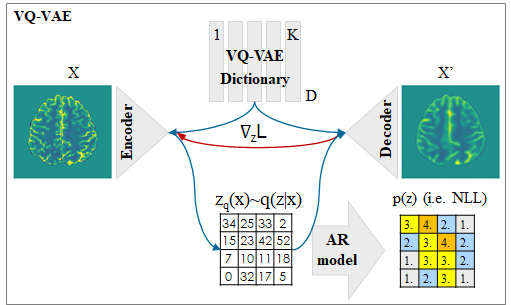
\includegraphics[width = 16cm, height = 6cm]{images/vqvae.png}
    \caption[]{VQ-VAE Proposed Approach by Marimont and Tarroni}
    \label{fig:vqvae}
\end{figure}

More recently, In September 2022, Soumick et al. published a paper on how a pipeline (called StRegA) with specific pre-processing and post-processing functions outperformed the Context-Encoder VAE (ceVAE) architectures on unsupervised anomaly detection in brain MRIs.

While Cardoso describes how a supercomputer with 100 GPUs (and other high-quality features) was employed to create MRI brain images across ages, genders and diseases which allows to not only diagnose but to predict diseases, StRegA describes how adding pre and post processing steps to the network architecture on regular computers improves results compared to bare VAE network architectures.

Soumick et al. explains in detail why the unsupervised learning is needed in the field by mainly comparing with supervised learning and by emphasizing its properties. The paper highlights the following list of reasons to justify the usage unsupervised learning:

\begin{itemize}
    \item Supervised learning relies on the quality and quantity of data, ranging from thousands to millions of labeled data which is a laborious manual annotation work.
    \item Supervised learning is often focused on one type of pathology
    \item Supervised learning has demonstrated to work well on concrete anomalies detection with simulated data but many perform poorly with clinical data
    \item Supervised learning solutions are challenging to develop on some abnormalities such as small vessel disease since the damage is complex on lesion size, contrast, or morphology
    \item A wide variety of abnormalities can be present in human brain MRI (even simultaneously) which renders a representation of all possible anomalies very challenging (including labeling)
    \item Anomaly detection is an approach that distinguishes anomalies completely based on characteristics that describe regular data.
    \item Unsupervised Anomaly Detection is useful for anomalies detection when their manifestation is not known or are very rare; making it difficult to create a large dataset for supervised learning
\end{itemize}

The StRegA pipeline used for unsupervised anomaly detection used a compact version of the ceVAE (cceVAE) combined with pre and post processors (creating a pipeline) which outperformed VAEs working alone. However, those achievements are only relevant to this project since they have been worked with the same MRI brain images (on a different dataset, BraTS vs IXI), hence it demonstrates that VAEs are optimal for MRI Brain images processing.

In conclusion, the state-of-the-art shows that VAEs have been implemented in combination with supercomputers to create models for diagnosis and prediction of brain diseases using 3-D MRI datasets and that the AI community is looking for cheaper and affordable implementations by innovating new VAE architectures or combining VAEs with pre and post processing actions.